\documentclass[
	12pt,
	oneside,
	a4paper,
	english,
	brazil
]{abntex2}

\usepackage{lmodern}
\usepackage[T1]{fontenc}
\usepackage[utf8]{inputenc}
\usepackage{indentfirst}
\usepackage{color}
\usepackage{graphicx}
\usepackage{microtype}
\usepackage{amsfonts}

\usepackage{caption}

\usepackage[brazilian,hyperpageref]{backref}
\usepackage[alf]{abntex2cite}

\usepackage{macros}

\titulo{Previsão de séries temporais por meio de aprendizado de máquina}
\autor{Guilherme Chichanoski}
\local{Maringá}
\data{2018}
\orientador{Valéria Delisandra Feltrim}
\instituicao{Universidade Estadual de Maringá\\
Centro de Tecnologia --- Departamento de Informática\\
Bacharelado em Ciência da Computação}
\tipotrabalho{Trabalho de Conclusão de Curso}

\preambulo{Trabalho de Conclusão de Curso de Graduação apresentado ao 
Departamento de Informática da Universidade Estadual de Maringá, como requisito 
parcial para obtenção do grau de Bacharel em Ciência da Computação.}

\makeatletter
\hypersetup{
		pdftitle={\@title},
		pdfauthor={\@author},
		pdfsubject={\imprimirpreambulo},
		pdfcreator={LaTeX with abnTeX2},
		pdfkeywords={abnt}{latex}{abntex}{abntex2}{projeto de pesquisa},
		colorlinks=true,	% false: boxed links; true: colored links
		linkcolor=blue,		% color of internal links
		citecolor=blue,		% color of links to bibliography
		filecolor=magenta,	% color of file links
		urlcolor=blue,
		bookmarksdepth=4
}
\makeatother

\setlength{\parindent}{1.3cm}
\setlength{\parskip}{0.2cm}

\begin{document}

\frenchspacing

\imprimircapa{}

\imprimirfolhaderosto{}

\textual{}

\pdfbookmark[0]{\contentsname}{toc}
\tableofcontents*
\cleardoublepage{}

\chapter{Introdução}

Segundo \citeonline{wiley} prever é a tarefa de predizer valores futuros ou 
eventos. Essa tarefa pode não ser trivial considerando que autores e 
organizações famosas já incorreram e ainda incorrem em previsões que se 
demonstram erradas, como exemplo podemos citar The New York Times que previu em 
1966 que em 2000 existiriam somente 220.000 computadores no Estados Unidos. A 
tarefa de prever é de grande importância para diversos setores incluindo 
governos e industrias, e sendo a atividade de previsão crucial para o apoio a 
tomada de decisão é evidente a necessidade de se realizar boas previsões.

Ainda segundo \citeonline{wiley} as previsões são classificas como sendo de 
curto, médio e longo prazo.  Sendo as de curto prazo previsões de um futuro 
próximo, ou seja, somente poucos passos a frente, podendo esses passos serem 
contados em dias, semanas ou meses.  Já previsões de médio prazo podem se 
estender por períodos de até um ano no futuro com os passos podendo ser dados em 
meses, enquanto que prazos mais longos serão chamados de previsões de longo 
prazo. Ainda conforme o autor, previsões de médio e longo prazo são mais 
difíceis e suscetíveis a fatores externos.

Para exemplificar a tarefa de previsão de curto prazo podemos citar a atividade 
de previsão da produção de energia eólica, como disposto em 
\citeonline{giebel2011state} a disponibilidade da energia produzida é dada 
segundo a capacidade do vento na região instalada, o vento no entanto é um 
elemento volátil e sendo assim se faz necessário se preparar para possíveis 
momentos onde se farão necessária o uso de outras fontes de energia, essa tarefa 
no entanto pode demandar conhecimento prévio pois o ligamento de uma usina como 
aquelas movidas a diesel podem levar até duas horas. Percebe-se então que a 
tarefa de prever duas horas a frente pode ser crucial para garantir o 
abastecimento de energia a uma região.

% FIXME: Tá esquisito
E em se tratando de previsões, uma fonte de informação comumente utilizado são 
as séries temporais, segundo \citeonline{wiley} essas séries são compostas de 
observações sequenciais ao longo do tempo. Por exemplo podemos observar o 
exemplo de série na figura-\ref{serie0}. Sendo essas observações separadas 
unicamente pelo tempo pode-se obter os dados em diferentes intervalos, como 
observações diárias, semanais ou ainda anuais.

\begin{figure}[ht]
    \centering
    \caption{Série gerada para exemplo}\label{serie0}
    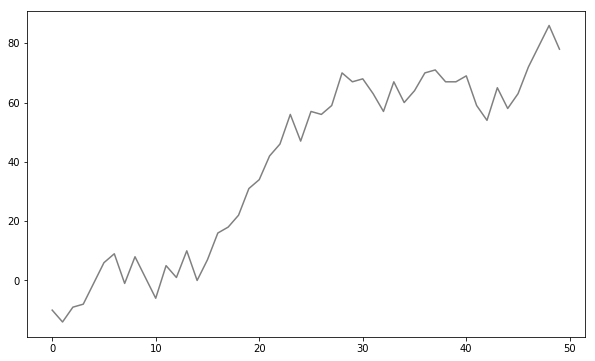
\includegraphics[width=.6\linewidth]{serie_exemplo.png}
    \source{Elaborado pelo autor}
\end{figure}

Tais séries possuem comportamento tal que permite a elaboração de um modelo que 
o representa de forma a permitir previsões, sendo os modelos estatísticos 
considerados os modelos mais comuns para esta finalidade. Como exemplo de 
aplicação podemos citar \citeonline{artigoEx1}, que obteve bons resultados em 
previsões de curto ao empregar modelos probabilísticos. Também vale a citar os 
resultados obtidos por \citeonline{artigoEx2}, onde também se empregou tais 
modelos e se obteve um modelo suficiente para realizações de previsões.

Em contrapartida podemos citar técnicas de aprendizado de máquinas que estão se 
tornando cada vez mais notórias pelos bons resultados que obtêm onde são 
aplicadas, como exemplo podemos citar o artigo de \citeonline{artigoEx3} onde a 
aplicação de modelos envolvendo aprendizado de máquina possibilitou a previsão 
com bons resultados. Pelo fato dos modelos estatísticos serem considerados quase 
um padrão para tais modelagens é comum que trabalhos como de 
\citeonline{artigoEx4} compare os resultados obtidos de modelos aprendizado com 
modelos de abordagem estatísticas. No caso dos modelos de aprendizado podemos 
citar como as redes neurais artificiais como sendo capaz de obter bons 
resultados conforme analisado por \citeonline{zhang}, o autor ainda apresenta 
outros exemplos onde a utilização de redes neurais obtiveram resultados 
superiores, considerando ainda que o estudo já está datado podemos encontrar em 
publicações recentes resultados ainda melhores.

A relevância das previsões são percebidas em aplicações onde esta é aplicada 
diretamente no processo de tomada de decisão, podendo auxiliar desde a 
organização de um negócio ao entendimento do comportamento de uma população.

\section{Previsão}
Segundo \citeonline{wiley} podemos separar o processo de previsão em diversas 
atividades, colocadas e detalhadas a seguir:

\begin{itemize}
	\item Definição do problema\\
		Envolve definir e entender a tarefa de previsão a ser realizada,
		considerando o prazo a ser previsto e definindo os dados necessários e
		quanto será o intervalo de uma previsão e outra.
	\item Coleta dos dados\\
		Conforme definido na etapa anterior ocorrerá nessa atividade a coleta
		dos dados.
	\item Análise dos dados\\
		Atividade de alta importância para a seleção do modelo mais adequado,
		nessa etapa é utilizada de observações gráficas e extração de dados para
		identificar padrões que ajudem. Ainda ocorrerá a identificação de 
		observações problemáticas e marcadas.
	\item Seleção e verificação do modelo\\
		Consiste da seleção e verificação de como o modelo escolhido se comporta 
		com os dados fornecidos. Para verificar o comportamento será utilizado 
		métricas que permitam comparar o resultado obtidos com outros modelos.
	\item Avaliação do modelo\\
		Etapa para avaliar como o modelo se comportará com novos dados obtidos, 
		normalmente é realizado a partir de dados separados obtidos das mesmas 
		informações utilizada em etapas anteriores, porem uma parte separada 
		somente para este fim.
	\item Publicação do modelo\\
		Com o modelo devidamente selecionado e avaliado o processo é instalado 
		em ambiente de produção, tendo que observar as alterações necessárias 
		para que novos dados sejam inseridos corretamente.
	\item Monitoramento da performance do modelo\\
		Uma ultima atividade que ocorrerá de forma recorrente, deve-se 
		continuamente avaliar como o modelo aplicado se comporta em relação ao 
		ambiente, já que o ambiente é algo volátil.
\end{itemize}

Vale-se notar que após a tarefa de avaliação se essa resultar em um valor 
insatisfatório deve-se retornar a fase anterior e refeita a avaliação até que um 
modelo que obedeça as especificações seja encontrado.

\section{Séries temporais}

Como já colocado anteriormente, séries temporais são observações sucessivas ao 
longo do tempo. Vale-se notar que esse tipo de série se caracteriza pelo fato de 
suas observações serem dependentes da observação anterior. Essas séries ainda 
podem demonstrar características como tendência e sazonalidade, sendo que a 
primeira confere a série um comportamento lento que pode levar a observações 
futuras como valores menores ou maiores e a segunda característica confere a ela 
padrão que apresente ciclos, podendo ser estes semanais, mensais, anuais ou um 
período qualquer de tempo.

Uma série é descrita matematicamente pelo conjunto $\{X(t): x \in T\}$, podendo 
ser $t$ um tempo contínuo ou discreto, sendo o primeiro quando se possui as 
observações de todos $t$ no conjunto dos $\mathbb{R}^{+}$ possíveis e a segunda 
quando entre uma observação e outra existe um intervalo igual de tempo.

Segundo \citeonline{ehlers} uma série temporal classicamente é decomposta 
seguindo a equação-\ref{eq:timeseries}, sendo $t$ usado para denotar o tempo, 
$T$ nos fornece a tendência e $C$ a componente sazonal ou cíclica, já $R$ é a 
componente aleatória e normalmente é caracterizada por possuir média zero, 
denota-se ainda como ruído branco.

\begin{equation}
	\label{eq:timeseries}
	X_t = T_t + C_t + R_t
\end{equation}

\subsection{Tendência}

Segundo \citeonline{ehlers} não existe uma definição precisa de tendência, mas 
normalmente é associado ao comportamento de mudança das observações em período 
de longo prazo. Uma série com tendência pode ser descrita como um função 
apresentada na equação-\ref{eq:tendencia}, $\alpha$ e $\beta{}$ coeficientes da 
função e $\epsilon{}_t$ o erro.

\begin{equation}
	\label{eq:tendencia}
	X_t = \alpha + \beta{}t + \epsilon{}_t
\end{equation}

Para exemplificar uma série temporal real podemos apresentar o gráfico na 
figura-\ref{fig:co2}, onde está apresentado a mudança na concentração de CO2 na 
atmosfera, no caso esta é uma série natural e demonstra evidentemente um 
comportamento tendencioso e com sazonalidade.

\subsection{Sazonalidade}

Conforme definido por \citeonline{ehlers} sazonalidade caracteriza repetições de 
comportamento de uma série em um período $s$ de tempo. Podemos expressar uma 
série sazonal usando a equação-\ref{eq:sazonal}

\section{Modelos probabilísticos}

Como já disposto, as séries temporais podem ser previstas utilizando de modelos 
estatísticos, isso segundo \citeonline{ehlers} ocorre devido ao seu caráter 
estocástico, ou seja, por conta de cada observação possuir correlação com as 
observações anteriores.

O modelo clássico utilizado para esse caso é o ARIMA, descrito por 
\citeonline{box}, descreve a série em três parâmetros $(p,d,q)$, sendo cada um 
associado a um processo, sendo $p$ associado a processos autoregressivos, $r$ a 
processos integrativos e $q$ a de médias móveis.

O processo autoregressivo 

\postextual

\bibliography{referencias}

\end{document}
